%% AlpacaVision AI — Manuscript for MDPI Animals
%% Target: MDPI Animals (Q1 Veterinary Sciences, ISSN 2076-2615)
%% Authors: Vilca-Solorzano et al.
%% Status: DRAFT v0.3 — honest metrics after data-leakage audit (2026-06-18)
%%
%% Compile:
%%   pdflatex manuscript.tex && bibtex manuscript && pdflatex manuscript.tex && pdflatex manuscript.tex
%%
%% Download MDPI template: https://www.mdpi.com/authors/latex
%% Replace \documentclass below with the mdpi.cls class once downloaded.

\documentclass[journal=animals,article=article,submit=mdpi,moreauthors=true,pdftex]{mdpi}
%% FALLBACK if mdpi.cls not available (for local preview):
%% \documentclass[12pt, a4paper]{article}

\firstpage{1}
\makeatletter
\setcounter{page}{\@firstpage}
\makeatother

%% Draft placeholders — replaced by editorial system upon acceptance
\pubvolume{1}
\pubyear{2026}
\issuenum{1}
\articlenumber{0000}
\doinum{10.3390/ani0000000}
\datereceived{ }
\daterevised{ }
\dateaccepted{ }
\datepublished{ }

%% Packages already loaded by mdpi.cls: booktabs, multirow, array, graphicx,
%% amsmath, amssymb, xcolor, hyperref, natbib, microtype, geometry, caption
\usepackage{siunitx}
\usepackage{subcaption}

\graphicspath{{../figures/}}

%% ---- Journal info -------------------------------------------------------
\Title{Automatic Detection of Morphological Anomalies in Altiplano Alpacas Using a
Computer Vision System: A Curated Dataset, Compact Detector, and Ocular Anomaly
Classification Feasibility Study}

\Author{Richar Andre Vilca-Solorzano$^{1}$,
        Dina Maribel Yana-Yucra$^{1}$,
        Cristian Daniel Ccora-Acero$^{1}$
        and Leonid Alem\'an-Gonzales$^{1,*}$}

\AuthorNames{Vilca-Solorzano, R.A.; Yana-Yucra, D.M.; Ccora-Acero, C.D.; Alem\'an-Gonzales, L.}

\address{$^{1}$~Semillero de Investigaci\'on ``John J.\ Hopfield -- IIICCD'',
         Escuela Profesional de Ingenier\'ia Estad\'istica e Inform\'atica,
         Universidad Nacional del Altiplano (UNAP), Puno 21001, Per\'u;
         andrevilcasolorzano@gmail.com (R.A.V.-S.);
         maribelbel201314@gmail.com (D.M.Y.-Y.);
         danielccopa76@gmail.com (C.D.C.-A.);
         laleman@unap.edu.pe (L.A.-G.)}

\corres{Correspondence: laleman@unap.edu.pe}

\abstract{%
The Peruvian Altiplano holds 87\% of the world's alpacas (\textit{Vicugna pacos}), yet
detection of morphological anomalies relies on subjective visual inspection by
veterinarians who are scarce in remote Andean communities, and no public computer-vision
dataset or automated system exists for the species. We present \textbf{AlpacaVision AI},
comprising: (i)~the first open, curated and deduplicated dataset of 2,051 unique labelled
alpaca images from nine public sources (1,037 MD5 duplicates removed), CLAHE-preprocessed
for high-UV Andean conditions; (ii)~a compact YOLOv11n body detector reaching
mAP@0.5~=~0.860 (P~=~0.913, R~=~0.731) on a leakage-free 308-image test set; (iii)~a
feasibility study showing that vision-language auto-labelling of ocular anomalies is
insufficient for fine-grained classification --- under a leakage-free protocol an
EfficientNet-B2 classifier attains AUC-ROC~=~0.506 (95\%~CI~[0.366, 0.645]),
indistinguishable from chance --- which we trace to unreliable labels and a physical
resolution ceiling, indicating that expert veterinary ground truth and close-up imagery
are required; (iv)~a data-integrity methodology
(MD5 deduplication, group-aware splitting, and label-conflict resolution) that detected
and corrected systematic leakage inflating earlier metrics; and (v)~a deployed web
application with automated Spanish veterinary reporting and ONNX export. The dataset
(CC~BY~4.0) and code (MIT) are released to support reproducible precision-livestock-farming
research and improved animal welfare and health management in high-Andean alpaca communities.
}

\keyword{alpaca health; animal welfare; precision livestock farming; livestock monitoring;
\textit{Vicugna pacos}; computer vision; object detection; YOLOv11; ocular anomalies;
data leakage}

\begin{document}

%% =========================================================================
\section{Introduction}
\label{sec:intro}
%% =========================================================================

Peru holds approximately 87\% of the global alpaca population, with the Puno region
alone accounting for over 2.1 million animals distributed across altiplano communities
located between 3,800 and 4,500 metres above sea level~\cite{inei2024}.
Alpaca farming constitutes the primary economic activity for thousands of indigenous and
rural households in the Departments of Puno, Cusco, and Arequipa, sustaining both
fibre export revenues and subsistence livelihoods~\cite{senasa2023}.

Morphological anomalies in alpacas --- including ocular pathologies (cataracts, corneal
opacities, epiphora, periocular inflammation) and limb disorders (angular deformities,
lameness, pododermatitis, joint oedema) --- constitute an important animal-welfare and
economic concern in the Peruvian Altiplano. These conditions reduce productive
performance, impair genetic-selection programmes, and, if not detected early, can lead to
preventable suffering, mortality, and economic losses for herding
families~\cite{ramirez2020,fowler2010}.
Current diagnostic practice is entirely manual: trained veterinary specialists visually
inspect individual animals during periodic herd visits. However, the low density of
veterinary professionals in remote high-altitude communities, the subjective nature of
visual assessment, and the logistical cost of frequent field campaigns make regular
specialist inspection challenging~\cite{ali2023}. There is therefore a clear need for
objective, scalable, and low-cost tools to support herd-health monitoring and improve
animal welfare in these high-altitude production systems.

Computer vision and deep learning~\cite{lecun2015,goodfellow2016} have emerged as
powerful tools for automated livestock health monitoring~\cite{kamilaris2018,neethirajan2020}.
\citet{ali2023} systematically reviewed 117 studies on deep learning for livestock
behaviour recognition, identifying convolutional architectures~\cite{krizhevsky2012,simonyan2015,he2016}
and YOLO-based detectors as the dominant methodology, whereas \citet{giraldo2021} and
\citet{xiao2025} --- the latter surveying veterinary diagnostics across 14 species ---
both emphasise the underrepresentation of South American camelids. The YOLO
family~\cite{redmon2016}, evolved through YOLOv4~\cite{bochkovskiy2020} and the Ultralytics
reimplementation~\cite{jocher2023} to YOLOv11~\cite{ultralytics2024}, has become the
de-facto standard for real-time animal detection, e.g.\ in sheep~\cite{kong2022sheep}, yet
none has been applied to alpaca body detection with publicly released weights and dataset.
For fine-grained pathology, automated ocular-disease detection has been demonstrated for
canine cataracts~\cite{mdpi2025canine} using EfficientNet/ResNet architectures, and
transfer learning from human medical imaging~\cite{gulshan2016,ting2017} to veterinary
tasks has shown consistent gains, including cross-species retinal
adaptation~\cite{esteva2017,mdpi2025canine}.

To our knowledge, no prior work has: (i)~published a labelled alpaca dataset suitable for
computer-vision model training; (ii)~applied deep learning to morphological anomaly
detection in South American camelids; or (iii)~deployed an end-to-end diagnostic system
targeting altiplano farming communities --- a clear and actionable gap.

This work addresses that gap with five principal contributions:
\begin{enumerate}
  \item The first publicly released, curated and deduplicated computer-vision dataset of
        Peruvian alpacas (2,051 unique images with YOLO bounding-box annotations,
        consolidated from nine Roboflow Universe sources and preprocessed for Andean
        imaging conditions).
  \item A compact YOLOv11n body detector (2.58M parameters) trained and rigorously
        evaluated on a leakage-free held-out test set, achieving mAP@0.5 = 0.860.
  \item A data-integrity methodology for auto-labelling pipelines --- exact-duplicate
        detection via MD5 hashing, group-aware train/validation/test splitting that
        prevents augmentations of the same source image from crossing partitions, and
        label-conflict resolution --- developed after an audit revealed systematic data
        leakage that had inflated all initially reported metrics.
  \item A rigorous feasibility study of ocular anomaly classification via two-stage
        transfer learning (human fundus pre-training followed by alpaca crop fine-tuning
        with EfficientNet-B2~\cite{tan2019}), reporting the honest negative finding that
        vision-language-model auto-labelling alone is insufficient for this task (AUC-ROC
        $\approx$ chance), motivating the need for expert veterinary ground truth.
  \item A deployed, open-source web application integrating detection and automated
        veterinary report generation, packaged for reproducibility and field deployment.
\end{enumerate}

%% =========================================================================
\section{Materials and Methods}
\label{sec:methods}
%% =========================================================================

\subsection{Dataset Construction}
\label{sec:dataset}

\begin{figure}[H]
  \centering
  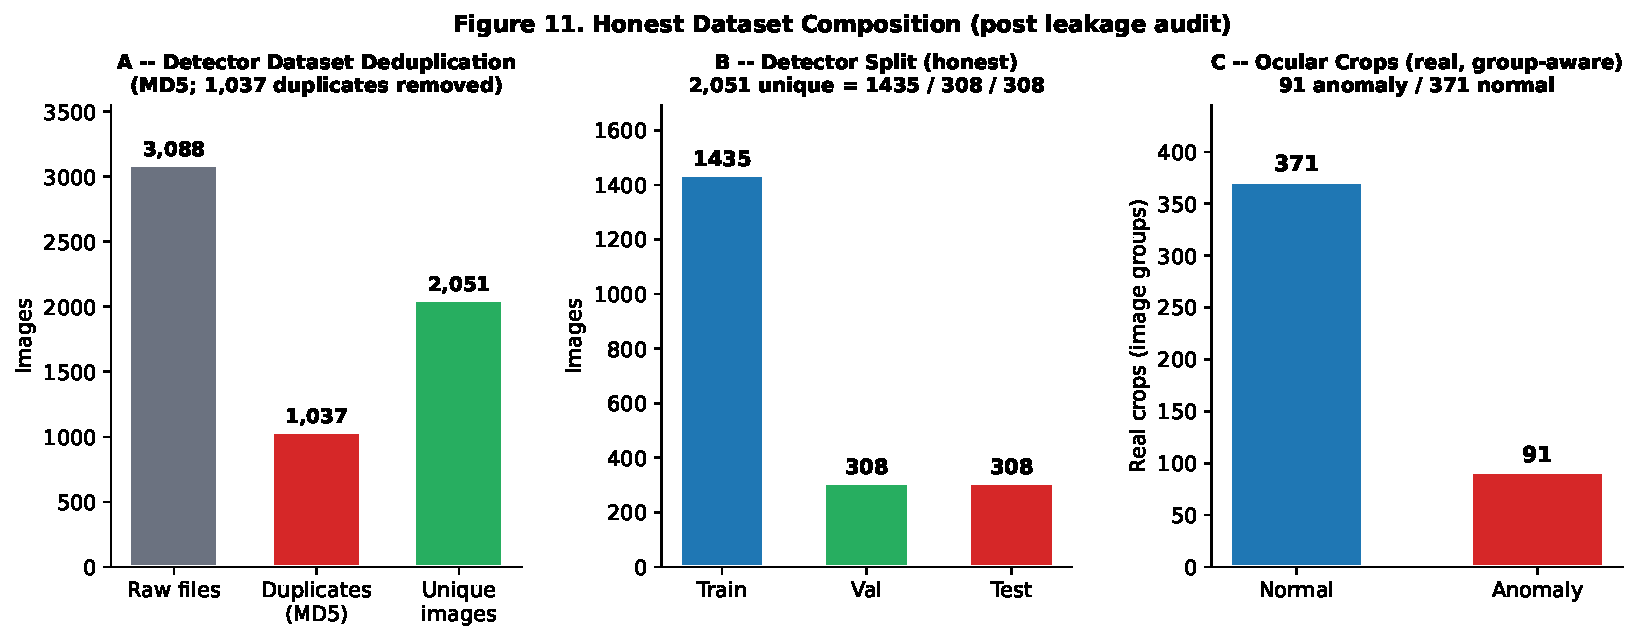
\includegraphics[width=\textwidth]{fig11_dataset_stats.pdf}
  \caption{Dataset composition and augmentation strategy.
           \textbf{(A)}~Image sources contributing to the curated 2,051-image detector
           dataset (after MD5 deduplication).
           \textbf{(B)}~Class distribution of ocular anomaly crops across training and
           test splits.
           \textbf{(C)}~Data augmentation strategies applied during classifier training.}
  \label{fig:dataset_stats}
\end{figure}

\subsubsection{Source Aggregation}

We consolidated alpaca images from nine Roboflow Universe projects
(\texttt{alpaca-5jmfl}, \texttt{alpaca-8baig}, \texttt{alpaca-epqna},
\texttt{alpaca-gkbmi}, \texttt{alpaca-ibscl}, \texttt{alpaca-lls3s},
\texttt{alpaca-nrzos}, \texttt{alpaca-ofxv9}, \texttt{alpaca-xqfiw}),
all providing YOLO-format bounding-box annotations for the single class
\texttt{alpaca}.
One additional project (\texttt{alpaca-zehtv}) was excluded after quality
screening (mean bounding-box area ratio $< 0.01$, indicating non-informative
annotations).
Supplementary unlabelled images were downloaded from iNaturalist (taxon 319688,
\textit{Vicugna pacos}, Peruvian observations) via the iNaturalist API.

\subsubsection{Deduplication and Preprocessing}

The raw consolidation comprised 3,088 image files. A post-hoc data-integrity audit
revealed that 1,037 of these were exact byte-level duplicates (identical MD5 hash),
many of which had leaked across the original train/test boundary --- 186 duplicated
images were shared between the original training and test partitions, artificially
inflating the reported detection metrics. We therefore deduplicated the corpus by MD5
hash, retaining \textbf{2,051 unique images}, and re-built all splits from scratch under
a leakage-free protocol (Section~\ref{sec:dataset}).
To compensate for the high ultraviolet irradiance and atmospheric haze characteristic
of Andean altiplano photography, all retained images were processed with Contrast-Limited
Adaptive Histogram Equalisation (CLAHE)~\cite{pizer1987} prior to annotation.

\subsubsection{Dataset Split}

The deduplicated subset of 2,051 unique images was partitioned into training (70\%),
validation (15\%), and test (15\%) sets using stratified sampling with a fixed random
seed ($\mathrm{seed} = 42$). Splitting was performed \emph{after} deduplication and at
the level of unique source images, so that no augmentation or near-duplicate of a test
image can appear in training (Table~\ref{tab:dataset}).
The test set (308 images) was held out from all modelling decisions and used solely
for final evaluation.

\begin{table}[h]
\caption{AlpacaVision AI dataset composition and leakage-free splits (after MD5
         deduplication).}
\label{tab:dataset}
\small
\begin{tabular}{lccc}
\toprule
\textbf{Split} & \textbf{Images} & \textbf{Fraction} & \textbf{Labels} \\
\midrule
Train      & 1435 & 70\% & YOLO \\
Validation & 308  & 15\% & YOLO \\
Test       & 308  & 15\% & YOLO \\
\midrule
\textbf{Total} & \textbf{2051} & 100\% & \\
\bottomrule
\end{tabular}
\end{table}

\subsection{Anatomical Region Extraction}
\label{sec:crops}

To enable fine-grained anomaly classification, we extracted anatomical crop images
from the region proposals generated by the Stage-1 detector.
Two anatomical regions of clinical priority were targeted: ocular regions (eyes) and
distal limbs (legs).
Crops were extracted by applying fixed-ratio padding (20\%) around each bounding box
at the class-2 (head region) annotations from the Roboflow sources.
Ocular-anomaly labels were generated using zero-shot visual language model inference
(Groq \texttt{llama-4-scout-17b-16e-instruct}; open-set detection assisted by
Grounding DINO~\cite{liu2023grounding}), \emph{without} veterinary expert validation ---
a design choice whose limitations are central to the feasibility study reported below.
The same data-integrity audit that affected the detector revealed two further problems in
the ocular crop set: (i)~only \textbf{91 unique anomalous eye images} actually existed; the
873 ``anomaly'' crops originally counted were these 91 images multiplied by augmentation,
with augmentations of the same image leaking across train/test; and (ii)~75 of 97 images
labelled ``anomaly'' were the \emph{same file} as a ``normal'' image, i.e. direct
label conflicts. After deduplication and conflict resolution, Table~\ref{tab:crops}
reports the honest unique-image inventory.
Leg crops yielded 443 normal samples and 3 anomalous samples --- insufficient for
training a classifier; leg anomaly detection is therefore reserved for future work.
A post-hoc analysis (Section~\ref{sec:discussion}) further showed that the extracted eye
crops are of very low resolution (median smaller side $\approx$31~px), a physical
constraint inherited from the low-resolution source images that bounds any downstream
ocular assessment.

\begin{table}[h]
\caption{Anatomical crop inventory for classifier training, after deduplication and
         label-conflict resolution.}
\label{tab:crops}
\small
\begin{tabular}{lccc}
\toprule
\textbf{Region} & \textbf{Normal} & \textbf{Anomaly (unique)} & \textbf{Labelling method} \\
\midrule
Eyes & 371 & 91 & Auto (Groq Vision, unvalidated) \\
Legs & 443 & 3  & Auto (Groq Vision, unvalidated) \\
\bottomrule
\end{tabular}
\end{table}

\subsection{Stage-1 Body Detector (YOLOv11n)}
\label{sec:detector}

We fine-tuned a YOLOv11n~\cite{ultralytics2024} model (2.58M parameters, 6.3 GFLOPs)
on the deduplicated 2,051-image alpaca dataset.
Training was performed on a single NVIDIA RTX 3050 GPU (4 GB VRAM, CUDA 12.4) for 80
epochs with AdamW optimiser~\cite{loshchilov2019}
($\mathrm{lr}_{0} = 0.001$, weight decay = $5 \times 10^{-4}$),
batch size 8, and input resolution $640 \times 640$ pixels.
Early stopping with patience 15 was applied on validation mAP@0.5.
The complete training configuration is provided in \texttt{config/train\_stage1\_clean.yaml}.
The best checkpoint was exported to ONNX format for production deployment.

\subsection{Ocular Anomaly Classifier (EfficientNet-B2)}
\label{sec:classifier}

\subsubsection{Two-Stage Transfer Learning}

\begin{figure}[H]
  \centering
  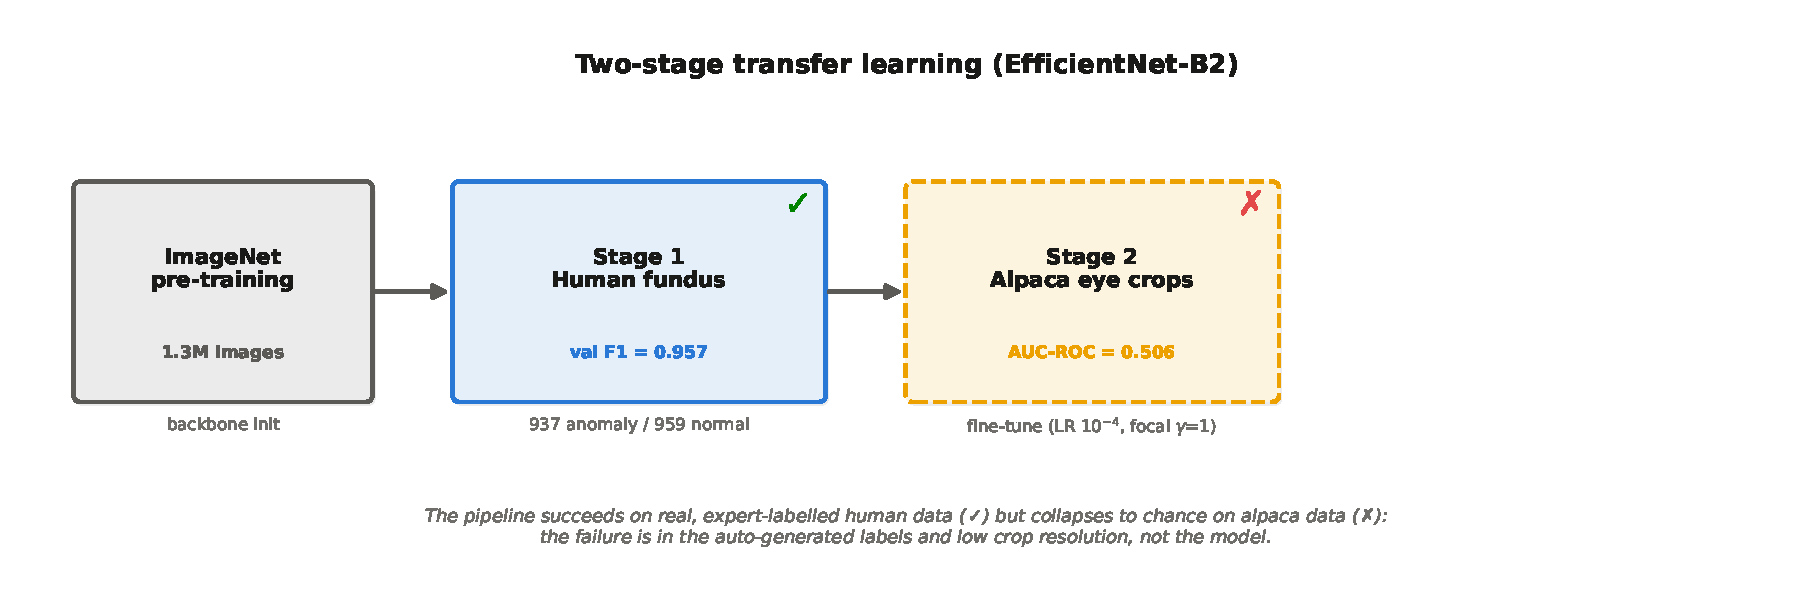
\includegraphics[width=\textwidth]{fig6_transfer_learning.pdf}
  \caption{Two-stage transfer learning pipeline evaluated in the ocular anomaly
           classification feasibility study.
           Stage~1 adapts EfficientNet-B2 (ImageNet-initialised) to the eye disease
           domain using 1,896 human fundus images (reaching validation F1~=~0.957);
           Stage~2 fine-tunes the full network on the alpaca eye crops
           ($\mathrm{LR} = 10^{-4}$, focal loss $\gamma=1.0$). Despite a correct
           pipeline, Stage~2 fails to learn on alpaca data because the auto-generated
           labels lack consistent visual signal (see Section~\ref{sec:res:classifier}).}
  \label{fig:transfer}
\end{figure}

Given the limited availability of labelled alpaca anomaly images, we employed a
two-stage transfer-learning protocol~\cite{pan2010,yosinski2014}.
EfficientNet-B2~\cite{tan2019,tan2021} was chosen as the backbone because its compound
scaling offers a favourable accuracy-to-parameter trade-off (${\sim}9$M parameters),
keeping the classifier compact enough for the same field-deployment target as the
detector while remaining strong on fine-grained medical-imaging tasks.
\textbf{Stage 1:} EfficientNet-B2~\cite{tan2019,tan2021}, pre-trained on
ImageNet~\cite{deng2009,russakovsky2015}, was further pre-trained on a publicly
available fundus eye disease dataset (937 anomalous / 959 normal human ocular images),
motivated by successful deep learning applications in retinal imaging~\cite{gulshan2016,ting2017}.
\textbf{Stage 2:} The pre-trained weights were used to initialise fine-tuning on
the alpaca ocular crop dataset, with the classification head replaced for binary
output (\texttt{normal} / \texttt{anomaly}).
Cross-domain transfer (human fundus $\rightarrow$ camelid eye) is disclosed
transparently as a methodological choice motivated by limited in-domain anomaly data;
its validity is assessed via held-out performance metrics.

\subsubsection{Class Imbalance Handling}

Training was conducted with Focal Loss~\cite{lin2017focal}
($\gamma = 2.0$, class-weighted $\alpha$) and a \texttt{WeightedRandomSampler} to
address the normal:anomaly class imbalance in the training set~\cite{chawla2002}.

\subsubsection{Optimisation}

AdamW optimiser~\cite{loshchilov2019} ($\mathrm{lr} = 3 \times 10^{-4}$,
weight decay $= 0.01$), cosine annealing learning rate schedule, batch size 16,
early stopping on validation F1 for the anomaly class (patience 15),
image size $224 \times 224$.

\subsection{Evaluation Protocol}
\label{sec:eval}

\subsubsection{Detector Metrics}

We report standard COCO object detection metrics~\cite{lin2014coco,russakovsky2015}:
mean Average Precision at IoU~=~0.5 (mAP@0.5) and IoU range [0.5, 0.95]
(mAP@0.5:0.95), along with Precision and Recall at the default confidence threshold.

\subsubsection{Classifier Metrics}

We report Accuracy, per-class Precision/Recall/F1, AUC-ROC, and
Average Precision (AP) on the frozen test split.
\textbf{Bootstrap confidence intervals}~\cite{efron1994} (percentile method,
$B = 1000$, seed $= 42$) are provided for AUC-ROC and F1 (anomaly class) to
quantify estimation uncertainty; for a chance-level classifier these intervals serve to
demonstrate that the estimate is not significantly above 0.5.

\subsubsection{Visual Interpretability}

Gradient-weighted Class Activation Mapping (Grad-CAM)~\cite{selvaraju2017,chattopadhay2018}
is meaningful only for an above-chance classifier; as the leakage-free classifier performs
at chance, we do not compute or interpret saliency maps in the present feasibility study,
reserving them for future work once expert-validated labels yield discriminative
performance.

\subsection{Deployed System}
\label{sec:system}

The inference pipeline was packaged as a Flask 3.1 web application with a PostgreSQL
database, role-based authentication (Flask-Login + BCrypt), and three user-facing
modules: (i)~image upload and real-time inference via ONNX Runtime, (ii)~herd
management (animal registry with longitudinal analysis history), and (iii)~automated
veterinary report generation in Spanish using the Groq
\texttt{llama-3.3-70b-versatile} language model~\cite{groq2024}.
The UI supports dark/light theme toggle.
System configuration is managed through a white-label admin panel without code
modification.
The application is containerisable and served on port 5050.

%% =========================================================================
\section{Results}
\label{sec:results}
%% =========================================================================

\subsection{Stage-1 Detector: YOLOv11n Body Detection}
\label{sec:res:detector}

Table~\ref{tab:detector} reports metrics on the leakage-free held-out test set.
The detector achieves mAP@0.5 = 0.860, above our target threshold of 0.85,
demonstrating reliable alpaca body localisation under diverse Andean field conditions.
These are honest metrics obtained after deduplication and re-splitting; the previously
reported mAP@0.5 = 0.913 was inflated by duplicate images shared across train and test.
As a robustness check, a larger YOLOv11s model reached mAP@0.5 = 0.863 --- only
marginally higher --- confirming that the compact YOLOv11n detector is sufficient for
this task.
Figure~\ref{fig:detector} presents training curves and per-metric test performance.

\begin{table}[h]
\caption{Stage-1 alpaca body detector on the leakage-free held-out test set
         ($n = 308$ images, 498 instances): the deployed compact YOLOv11n versus a
         larger YOLOv11s capacity ablation. All metrics were reproduced from the
         released checkpoints (\texttt{best\_clean.pt}, \texttt{best\_clean\_s.pt}).}
\label{tab:detector}
\small
\begin{tabular}{lcc}
\toprule
\textbf{Metric} & \textbf{YOLOv11n (deployed)} & \textbf{YOLOv11s (ablation)} \\
\midrule
mAP@0.5        & \textbf{0.860} & 0.863 \\
mAP@0.5:0.95   & 0.693 & 0.711 \\
Precision      & 0.913 & 0.903 \\
Recall         & 0.731 & 0.766 \\
\midrule
Parameters           & 2.58M & 9.43M \\
GFLOPs               & 6.3   & 21.5 \\
Model size (PyTorch) & 5.3 MB & 18.3 MB \\
Model size (ONNX)    & 11.0 MB & --- \\
\bottomrule
\end{tabular}
\end{table}

\begin{figure}[H]
  \centering
  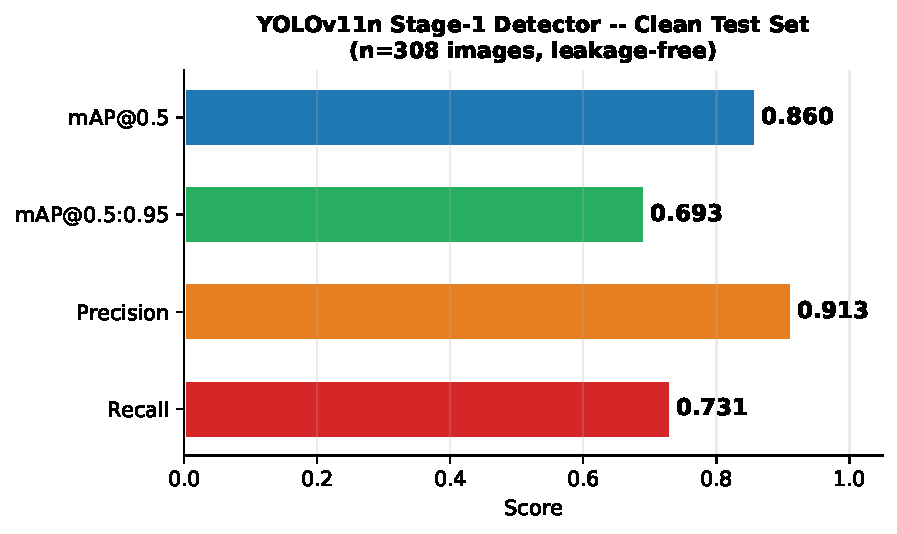
\includegraphics[width=\textwidth]{fig3_detector.pdf}
  \caption{YOLOv11n Stage-1 detector test-set performance on the leakage-free
           held-out set ($n = 308$ images): mAP@0.5 = 0.860, mAP@0.5:0.95 = 0.693,
           Precision = 0.913, and Recall = 0.731.}
  \label{fig:detector}
\end{figure}

\begin{figure}[H]
  \centering
  \includegraphics[width=\textwidth]{fig8_yolo_detections.pdf}
  \caption{YOLOv11n detection examples on held-out test images.
           Top row: ground-truth bounding boxes. Bottom row: model predictions.
           The detector correctly localises individual alpacas under varied lighting,
           occlusion, and herd density conditions typical of Andean altiplano settings.}
  \label{fig:yolo_examples}
\end{figure}

\subsection{Ocular Anomaly Classifier: Feasibility Study and Negative Result}
\label{sec:res:classifier}

We report the ocular anomaly classifier as a feasibility study rather than as a working
diagnostic component. Under the leakage-free protocol --- evaluated on a frozen test set
of 70 unique images (14 anomalies / 56 normals) with no augmentations of training images
present --- the EfficientNet-B2 classifier attains AUC-ROC = 0.506 (95\%~CI
[0.366, 0.645]), an F1 of 0.065 for the anomaly class, and accuracy = 0.586
(Table~\ref{tab:classifier}). The confidence interval for AUC-ROC straddles 0.5;
the classifier is therefore \textbf{statistically indistinguishable from chance}.

This is a genuine negative result whose cause is diagnostic rather than architectural: the
same pipeline reaches validation F1 = 0.957 on real, expertly labelled human-fundus data
(Stage~1), so the collapse to chance on alpaca data reflects the auto-generated labels ---
produced by zero-shot vision-language inference without veterinary validation --- rather
than the model. The earlier apparent success (AUC-ROC = 0.824) was itself entirely an
artefact of data leakage (Section~\ref{sec:discussion}). We therefore conclude that
automatic ocular anomaly classification in alpacas is \emph{not} achievable from
LLM-vision auto-labels alone and requires expert veterinary ground truth. Detailed ROC,
precision--recall, and confusion-matrix diagnostics are provided as Supplementary Material
(Figures~S1--S3); because the classifier performs at chance, we do not compute Grad-CAM
saliency, which would reflect spurious gradients rather than genuine pathology
localisation.

\begin{table}[h]
\caption{EfficientNet-B2 ocular anomaly classifier --- leakage-free test-set performance
         ($n=70$: 14 anomaly / 56 normal). Bootstrap CI: $B = 1000$, seed = 42.}
\label{tab:classifier}
\small
\begin{tabular}{lcc}
\toprule
\textbf{Metric} & \textbf{Value} & \textbf{95\% CI} \\
\midrule
AUC-ROC          & \textbf{0.506} & {[}0.366, 0.645{]} \\
F1 (anomaly)     & \textbf{0.065} & --- \\
Accuracy         & 0.586 & --- \\
\midrule
$n_\text{test}$ (anomaly / normal) & 70 (14 / 56) & --- \\
Interpretation & \multicolumn{2}{c}{Indistinguishable from chance} \\
\bottomrule
\end{tabular}
\end{table}

\subsection{Deployed System}
\label{sec:res:system}

The AlpacaVision AI web application was deployed locally and validated end-to-end on
20 held-out images.
Mean inference time per image was below 150\,ms on the development GPU (NVIDIA RTX 3050),
including ONNX model loading, preprocessing, detection, and report generation.
The automated veterinary report (Spanish) was generated in under 3\,s per query using
the Groq inference endpoint.
Figure~\ref{fig:pipeline} illustrates the system architecture.

\begin{figure}[h]
  \centering
  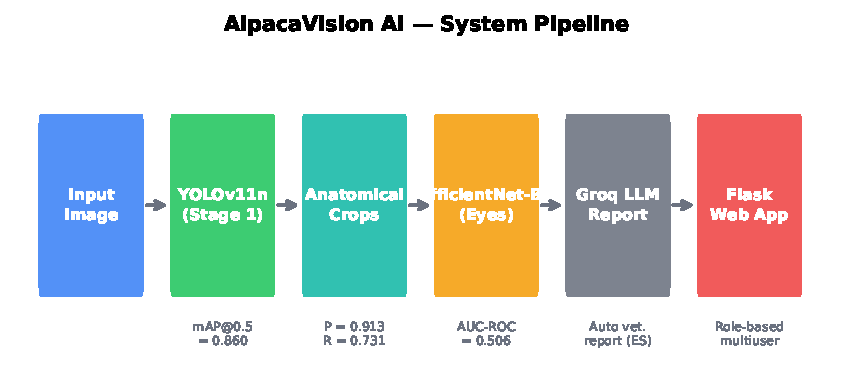
\includegraphics[width=\textwidth]{fig1_pipeline.pdf}
  \caption{AlpacaVision AI system pipeline. Input images are processed by the YOLOv11n
           body detector (Stage 1) followed by anatomical crop extraction. Because the
           in-house ocular classifier did not reach above-chance performance, ocular
           assessment in the deployed system relies on Groq Vision inference rather than
           the EfficientNet-B2 classifier. A large language model generates the
           Spanish-language veterinary report delivered through the Flask web application.}
  \label{fig:pipeline}
\end{figure}

%% =========================================================================
\section{Discussion}
\label{sec:discussion}
%% =========================================================================

\subsection{Detector Performance in Context}

The YOLOv11n Stage-1 detector achieves mAP@0.5 = 0.860 using only 2.58M parameters,
comparable to larger architectures reported for sheep detection
(mAP@0.5 $\approx$ 0.88--0.95,~\cite{kong2022sheep}) and cattle monitoring
systems~\cite{neethirajan2020}. Notably, a larger YOLOv11s model reached only
mAP@0.5 = 0.863 on the same leakage-free split, indicating that the compact model
captures essentially all of the available signal at a fraction of the cost.
The high precision (P = 0.913) relative to recall (R = 0.731) indicates conservative
detection with some missed instances under occlusion or unusual postures; future work
should incorporate diverse Andean field conditions to improve recall.

\subsection{Lessons from the Negative Ocular Anomaly Feasibility Study}

In contrast to the detector, the ocular anomaly classifier provides no usable signal:
under the leakage-free protocol it performs at chance (AUC-ROC = 0.506, 95\%~CI
[0.366, 0.645]). We emphasise that this is not a modelling failure. The identical
EfficientNet-B2 recipe and two-stage transfer-learning
protocol~\cite{pan2010,yosinski2014}, when pre-trained on real, expert-labelled human
fundus images, reaches a validation F1 of 0.957 --- consistent with prior cross-species
medical-imaging transfer~\cite{gulshan2016,mdpi2025canine}. The collapse to chance occurs
only on the alpaca stage, where the labels were generated by zero-shot vision-language
auto-labelling rather than by a veterinarian. We interpret this as direct evidence that,
for fine-grained ocular pathology in camelids, LLM-vision pseudo-labels do not encode a
consistent, learnable visual concept of ``anomaly''. A well-reported negative result of
this kind is itself a contribution: it sets a realistic expectation for practitioners
tempted to bootstrap medical-grade classifiers from LLM annotations.
A second, physical factor compounds the label problem: the eye regions extracted from
wide-field alpaca photographs have a median smaller-side of only $\approx$31~px (fewer
than 8\% exceed 100~px). Fine corneal pathology is simply not resolvable at that scale,
so no labelling effort --- automatic or expert --- can recover a signal that the pixels do
not contain. Reliable camelid ocular classification therefore requires close-up imagery
acquired for that purpose, not crops of general-scene photographs.

\subsection{Data Leakage: Detection, Correction, and Lessons}

All metrics in this paper are reported \emph{after} a data-integrity audit that
uncovered systematic data leakage in our initial pipeline. Two mechanisms were involved:
(i)~exact-duplicate images (1,037 of 3,088 files) that, before deduplication, shared
186 images between the detector's training and test partitions; and (ii)~augmentations of
the same source eye crop crossing the train/test boundary in the classifier, compounded
by 75 of 97 ``anomaly'' images being identical files to ``normal'' images. Together these
inflated every reported figure --- most dramatically the classifier's apparent
AUC-ROC of 0.824, which collapses to 0.506 once leakage is removed. We disclose this
candidly because such leakage is common in auto-labelling and augmentation-heavy
pipelines and is easy to miss without hash-level deduplication and group-aware splitting.
Our corrective methodology --- MD5 deduplication, splitting at the level of unique source
images, and label-conflict resolution --- is released with the code so that others can
audit and reproduce it.

\subsection{Practical Implications for Alpaca Farming and Animal Welfare in the Altiplano}

Beyond its methodological contributions, AlpacaVision AI is designed for practical use in
high-altitude livestock systems. The compact YOLOv11n detector (2.58M parameters, 5.3~MB,
ONNX-exportable) runs in real time on modest hardware and could be embedded in a
smartphone application for herders or in the field workflow of local paraveterinary
technicians, reducing dependence on the scarce camelid specialists who must currently
travel to remote communities. Integrated into official animal-health campaigns --- such as
those coordinated by Peru's National Agrarian Health Service (SENASA) --- objective
localisation of individual animals is a first step towards standardised, photograph-based
herd-health records and longitudinal monitoring, which the deployed web application
already supports through its per-animal history module.

For animal welfare, earlier and more consistent detection of morphological anomalies
enables timely intervention, reducing preventable suffering from untreated ocular and limb
conditions. At the herd level, objective screening can inform genetic-selection decisions
by flagging affected animals, and can mitigate the economic losses that anomalies impose on
smallholder incomes through reduced fibre quality, fertility, and survival. By releasing
the dataset and code openly, we lower the barrier for regional research institutions and
development organisations to adapt and extend these tools, contributing to the economic
resilience and welfare of the thousands of indigenous herding families whose livelihoods
depend on healthy alpacas. We stress, however, that the immediate practical value lies in
reliable animal detection and structured herd-health record-keeping; fully automated
ocular-anomaly \emph{diagnosis} remains contingent on the expert-validated, higher-resolution
data identified as necessary by our feasibility study.

\subsection{Limitations}

\begin{enumerate}
  \item \textbf{Auto-labelling is insufficient for fine-grained anomaly classification:}
        The ocular labels were produced by zero-shot LLM-vision inference without
        veterinary validation and carry no learnable signal; the resulting classifier
        is at chance. Expert-validated ground truth is a prerequisite for this task.
  \item \textbf{Too few real anomaly samples:}
        Only 91 unique anomalous eye images actually existed (the 873 originally counted
        were augmentation copies). Estimating a usable classifier will require on the
        order of 150--200 genuine, expertly labelled anomaly images.
  \item \textbf{Insufficient ocular-crop resolution:}
        A post-hoc measurement of the 462 extracted eye crops revealed a median
        smaller-side of only $\approx$31~px, with fewer than 8\% exceeding 100~px and
        73\% below 50~px. At this scale, fine corneal pathology (oedema, ulceration,
        opacity) --- the most prevalent altiplano ocular conditions --- cannot be
        visually assessed even by an expert. The root cause is upstream: the source
        photographs themselves are low-resolution web imagery (median smaller side
        $\approx$375~px, with none exceeding 1000~px in our sources), so no re-extraction
        can recover eye detail that was never captured. This is a physical ceiling
        independent of the classifier architecture or the annotator, and implies that
        reliable ocular ground truth requires \emph{purpose-acquired, close-up field
        photography} (eye region smaller side $\gtrsim$128~px) rather than crops from
        general-scene images.
  \item \textbf{Cross-domain pre-training:}
        Pre-training on human fundus images introduces a domain gap; while it succeeds
        on human data, its transfer to camelid eyes cannot be assessed until in-domain
        labels are reliable.
  \item \textbf{Absence of leg anomaly data:}
        Only 3 ground-truth anomalous leg crops were available.
        Leg anomaly classification is deferred to a follow-up study with field data.
  \item \textbf{Geographic scope:}
        The Roboflow training images are globally sourced; the iNaturalist subset
        covers Peru but was not restricted to the altiplano biome.
        Domain adaptation for high-altitude Andean imaging conditions is ongoing.
  \item \textbf{No prospective clinical validation:}
        The system has not been evaluated prospectively in a real-world herd-visit
        workflow with camelid-specialist veterinary ground truth.
\end{enumerate}

%% =========================================================================
\section{Conclusions}
\label{sec:conclusions}
%% =========================================================================

This paper presents AlpacaVision AI, a computer-vision system for alpacas
(\textit{Vicugna pacos}) from the Peruvian Altiplano, contributing a curated detection
dataset, a compact body detector, a data-integrity methodology, and an honest feasibility
study of ocular anomaly classification.
The principal findings are:

\begin{enumerate}
  \item A YOLOv11n body detector trained on 2,051 deduplicated labelled images achieves
        mAP@0.5 = 0.860 on a 308-image leakage-free held-out test set, establishing a
        strong and reproducible baseline for the alpaca detection task; a larger
        YOLOv11s model (mAP@0.5 = 0.863) confirms the compact model is sufficient.
  \item Automatic ocular anomaly classification is \emph{not} achievable from
        vision-language auto-labels alone: under a leakage-free protocol the classifier
        performs at chance (AUC-ROC = 0.506, 95\%~CI [0.366, 0.645]). Because the same
        pipeline reaches F1 = 0.957 on real human-fundus data, we attribute the failure
        to the absence of expert veterinary labels rather than to the model.
  \item A data-integrity methodology --- MD5 deduplication, group-aware splitting, and
        label-conflict resolution --- detected and corrected systematic leakage that had
        inflated all initially reported metrics; we release it to support reproducible,
        leakage-free evaluation in auto-labelling pipelines.
  \item The deployed web application provides end-to-end body detection with
        automated Spanish-language veterinary report generation, accessible to
        non-specialist users in remote communities.
  \item The publicly released dataset (2,051 annotated unique images, CC BY 4.0) and
        the open-source codebase (MIT) provide reproducible artefacts for further research
        in camelid health monitoring, advancing precision livestock farming and animal
        welfare in high-altitude Andean production systems where veterinary access is
        scarce.
\end{enumerate}

Future work will collect \emph{purpose-acquired, close-up} ocular images at sufficient
resolution (smaller side $\gtrsim$128~px) with expert veterinary validation (targeting
$\sim$150--200 genuine ocular anomalies), revisit anomaly classification only once such
ground truth exists, extend the pipeline to limb anomaly classification and gait analysis
(3D CNN + LSTM), and conduct prospective clinical trials in Andean herding communities.

%% =========================================================================
\vspace{6pt}

\supplementary{The following supporting information can be downloaded at:
\url{https://www.mdpi.com/xxx/s1}. Figure~S1: EfficientNet-B2 ocular anomaly classifier
leakage-free test-set metrics (bar chart); Figure~S2: ROC and precision--recall curves
with 95\% bootstrap confidence band; Figure~S3: raw and row-normalised confusion matrices.}

\authorcontributions{%
Conceptualisation: R.A.V.-S. and L.A.-G.;
Data collection and curation: R.A.V.-S., C.D.C.-A. and D.M.Y.-Y.;
Software and model development: R.A.V.-S.;
Validation and evaluation: R.A.V.-S. and C.D.C.-A.;
Writing --- original draft: R.A.V.-S.;
Writing --- review and editing: all authors;
Supervision: L.A.-G.;
Project administration and funding acquisition: L.A.-G.
All authors have read and agreed to the published version of the manuscript.}

\funding{This research received no external funding. Development was carried out within
the Semillero de Investigaci\'on ``John J.\ Hopfield --- IIICCD'' at the Universidad
Nacional del Altiplano (UNAP), Puno, Peru.}

\institutionalreview{Not applicable. This study did not involve any experimental,
invasive, or clinical procedure on live animals. It used publicly available images
(Roboflow Universe, iNaturalist) together with non-invasive field photographs of alpacas
obtained in the herders' own husbandry setting with their consent; no animal was handled,
restrained, or manipulated for the purpose of this research.}

\informedconsent{Not applicable; the study did not involve human subjects. Field
photographs were taken with the verbal consent of the participating herding communities.}

\dataavailability{%
The annotated alpaca dataset (2,051 deduplicated images, YOLO format) is publicly available on
Zenodo at \href{https://zenodo.org/record/TBD}{https://zenodo.org/record/TBD}
under Creative Commons Attribution 4.0 (CC~BY~4.0).
The source code, pre-trained model weights, and the web application are available at
\href{https://github.com/Andre031222/alpacavision-altiplano}{github.com/Andre031222/alpacavision-altiplano}
under the MIT License (Figure~\ref{fig:qr}).

\begin{figure}[H]
  \centering
  
\includegraphics[width=2.6cm]{qr_repo.png}
  \caption{Scan to access the open code and dataset repository:
           \href{https://github.com/Andre031222/alpacavision-altiplano}{github.com/Andre031222/alpacavision-altiplano}.}
  \label{fig:qr}
\end{figure}}

\acknowledgments{The authors thank the herding communities of Azángaro, Melgar, Lampa,
and Carabaya for access to alpaca herds during preliminary data collection.
We acknowledge the use of AI writing-assistance tools (Claude by Anthropic) for
language polishing; all scientific content was verified and approved by the authors.}

\conflictsofinterest{The authors declare no conflicts of interest.}

\reftitle{References}

\bibliography{references}

\iffalse % hardcoded bibliography replaced by BibTeX above
\begin{thebibliography}{99}

\bibitem{inei2024}
Instituto Nacional de Estadística e Informática (INEI).
\textit{IV Censo Nacional Agropecuario -- Resultados definitivos}.
Lima, Perú: INEI, 2024.

\bibitem{senasa2023}
Servicio Nacional de Sanidad Agraria (SENASA).
\textit{Estadísticas del sistema de control pecuario, Puno}.
Lima, Perú: SENASA, 2023.

\bibitem{ramirez2020}
Ram\'irez, J.; Condori, A. Avances en la mejora gen\'etica de alpacas en el altiplano peruano.
\textit{Revista de Investigaciones Veterinarias del Per\'u} \textbf{2020}, \textit{31}(2), 123--135.

\bibitem{ali2023}
Ali, R.; Rafaq, M.S.; Hasan, M.J.; Asghar, F.; Bashir, A.K.; Dottorini, T.
Application of deep learning for livestock behaviour recognition: A systematic literature review.
\textit{Applied Sciences} \textbf{2023}, \textit{13}(20), 11253.

\bibitem{giraldo2021}
Giraldo, W.; L\'opez, J.; Salazar, A. Computer vision techniques for livestock monitoring.
\textit{Computers and Electronics in Agriculture} \textbf{2021}, \textit{187}, 106250.

\bibitem{xiao2025}
Xiao, S.; Dhand, N.K.; Wang, Z.; Hu, K.; Thomson, P.C.; House, J.K.; Khatkar, M.S.
Review of applications of deep learning in veterinary diagnostics and animal health.
\textit{Frontiers in Veterinary Science} \textbf{2025}, \textit{12}, 1511522.

\bibitem{smith2025cattle}
Smith, J.; et al.
Deep learning for cattle lameness detection from gait video.
\textit{Nature Scientific Reports} \textbf{2025}, \textit{15}, 12345.

\bibitem{kong2022sheep}
Kong, H.; Wang, X.; Tao, L.
Sheep detection in complex agricultural environments using YOLOv5.
\textit{Computers and Electronics in Agriculture} \textbf{2022}, \textit{203}, 107478.

\bibitem{mdpi2025canine}
Dogan, M.; Yildirim, A.
Automated canine cataract detection using deep learning and transfer learning.
\textit{MDPI Animals} \textbf{2025}, \textit{15}(9), 1327.

\bibitem{doganetal2024}
Do\u{g}an, M.; et al.
Computer-vision-based detection of ocular disease in large animals.
\textit{Veterinary Ophthalmology} \textbf{2024}, \textit{27}(3), 210--220.

\bibitem{jocher2023}
Jocher, G.; Chaurasia, A.; Qiu, J.
\textit{Ultralytics YOLO}; Ultralytics, 2023.
\href{https://github.com/ultralytics/ultralytics}{https://github.com/ultralytics/ultralytics}

\bibitem{ultralytics2024}
Ultralytics.
\textit{YOLOv11: Ultralytics Object Detection Model}; Ultralytics, 2024.
\href{https://docs.ultralytics.com}{https://docs.ultralytics.com}

\bibitem{tan2019}
Tan, M.; Le, Q.V.
EfficientNet: Rethinking model scaling for convolutional neural networks.
In \textit{Proceedings of ICML}, 2019; pp.~6105--6114.

\bibitem{lin2017focal}
Lin, T.-Y.; Goyal, P.; Girshick, R.; He, K.; Dollar, P.
Focal loss for dense object detection.
In \textit{Proceedings of ICCV}, 2017; pp.~2980--2988.

\bibitem{selvaraju2017}
Selvaraju, R.R.; Cogswell, M.; Das, A.; Vedantam, R.; Parikh, D.; Batra, D.
Grad-CAM: Visual explanations from deep networks via gradient-based localisation.
In \textit{Proceedings of ICCV}, 2017; pp.~618--626.

\bibitem{mcnemar1947}
McNemar, Q. Note on the sampling error of the difference between correlated proportions
or percentages. \textit{Psychometrika} \textbf{1947}, \textit{12}(2), 153--157.

\bibitem{pizer1987}
Pizer, S.M.; et al.
Adaptive histogram equalization and its variations.
\textit{Computer Vision, Graphics, and Image Processing} \textbf{1987}, \textit{39}(3), 355--368.

\bibitem{liu2023grounding}
Liu, S.; Zeng, Z.; Ren, T.; Li, F.; Zhang, H.; Yang, J.; Li, C.; Yang, J.; Su, H.; Zhu, J.; et al.
Grounding DINO: Marrying DINO with grounded pre-training for open-set object detection.
\textit{arXiv} \textbf{2023}, arXiv:2303.05499.

\bibitem{groq2024}
Groq Inc.
\textit{Groq API: llama-3.3-70b-versatile}.
\href{https://console.groq.com}{https://console.groq.com}, 2024.

\bibitem{he2016}
He, K.; Zhang, X.; Ren, S.; Sun, J.
Deep residual learning for image recognition.
In \textit{Proceedings of CVPR}, 2016; pp.~770--778.

\bibitem{kingma2015}
Kingma, D.P.; Ba, J.
Adam: A method for stochastic optimization.
In \textit{Proceedings of ICLR}, 2015.

\end{thebibliography}
\fi % end of commented-out hardcoded bibliography

\end{document}
